\documentclass[12pt]{article}
\usepackage[english]{babel}
\usepackage{natbib}
\usepackage{url}
\usepackage[utf8x]{inputenc}
\usepackage{amsmath}
\usepackage{graphicx}
\graphicspath{{images/}}
\usepackage{parskip}
\usepackage{fancyhdr}
\usepackage{vmargin}
\setmarginsrb{3 cm}{2.5 cm}{3 cm}{2.5 cm}{1 cm}{1.5 cm}{1 cm}{1.5 cm}

% Template started from: https://www.overleaf.com/latex/templates/uct-report-template/grctkzjtrqrm

\title{Course Project}										% Title
\author{Grant Atkins\\David Haslam}							%Authors
\date{\today}											% Date

\makeatletter
\let\thetitle\@title
\let\theauthor\@author
\let\thedate\@date
\makeatother

%\pagestyle{fancy}
%\fancyhf{}
%\rhead{\theauthor}
%\lhead{\thetitle}
%\cfoot{\thepage}

\begin{document}

%%%%%%%%%%%%%%%%%%%%%%%%%%%%%%%%%%%%%%%%%%%%%%%%%%%%%%%%%%%%%%%%%%%%%%%%%%%%%%%%%%%%%%%%%

\begin{titlepage}
	\centering
    \vspace*{0.5 cm}
    
\includegraphics[scale = 1.8]{ODU.png}\\[1.0 cm]	% University Logo
    \textsc{\LARGE Old Dominion University}\\[2.0 cm]	% University Name
	\textsc{\Large CS 773}\\[0.5 cm]				% Course Code
	\textsc{\large Data Mining and Security}\\[0.5 cm]				% Course Name
	\rule{\linewidth}{0.2 mm} \\[0.4 cm]
	{ \huge \bfseries \thetitle}\\
	\rule{\linewidth}{0.2 mm} \\[1.5 cm]
	
	\begin{minipage}{0.4\textwidth}
		\begin{flushleft} \large
			\emph{Authors:}\\
			\theauthor
			\end{flushleft}
			\end{minipage}~
			\begin{minipage}{0.4\textwidth}
			\begin{flushright} \large
%			\emph{Student Number:} \\
%			XXXXXX000									% Your Student Number
		\end{flushright}
	\end{minipage}\\[2 cm]
	
	{\large \thedate}\\[2 cm]
 
	\vfill
	
\end{titlepage}

%%%%%%%%%%%%%%%%%%%%%%%%%%%%%%%%%%%%%%%%%%%%%%%%%%%%%%%%%%%%%%%%%%%%%%%%%%%%%%%%%%%%%%%%%

\tableofcontents
\pagebreak

%%%%%%%%%%%%%%%%%%%%%%%%%%%%%%%%%%%%%%%%%%%%%%%%%%%%%%%%%%%%%%%%%%%%%%%%%%%%%%%%%%%%%%%%%

\section{Executive Summary}

The goal of this course project, originally stemmed from Open University Learning Analytics dataset, is to identify `at-risk` students 
provided \cite{oulad}.

More needs to be done in this section...

%This is a simple report template with the UCT logo. Feel free to use/modify it to suit your needs. Variables that need to be altered have been commented to make modifications easier. For example if you need to change the university logo, look for the comment \texttt{\% University Logo} in this file and then make appropriate modifications in that line.
%
%A Table of Contents and a bibliography have also been implemented. To add entries to your bibliography, simply edit \texttt{biblist.bib} in the root folder and then use the \texttt{\textbackslash cite\{\ldots\}} command in \texttt{main.tex} \cite{bibtex}. The Table of Contents will be updated automatically.
%
%I hope that you find this template both visually appealing and useful. \\

\section{Introduction}

With analytics becoming an integral part of Learning Management Systems (LMS), Universities can analyze their data to intervene and aid `at-risk` 
students. This can be done by detecting failing or struggling students earlier on in their courses. These detections can later be used to predict `at-risk`
students for future intervention. Analysis of demographic information for students may also prove useful to detect environments or character
attributes that identify a struggling group.

The Open University (OU) in the United Kingdom, offered distance learning courses with its virtual learning environment (VLE) from 2013 to 2014. Students interacted with 
the VLE and OU then collects information such as: page names, clicks, and times connected to the website. Students are also required to register for these 
courses earlier on, which provides: registration date, unregistration date, class types and semester. Many students may end fail or withdraw from the VLE 
courses. The datasets that OU provided can be used to provide insight on 2013 to 2014 semester students. 

\section{Problem Statement}

When analyzing students to observe for `at-risk` students it may seem easily done by looking at simply grade scores, however, there could be independent factors
present in a student's personal history or personal accomplishments that cause a student to be `at-risk.` The goal of this paper is discuss and find data mining techniques that aid
in the detection and prediction of `at-risk` students.

\section{Solution Methodology}

Finding a solution for this project was based on the data being observed. We first attempted to look at each dataset, each csv provided, individually and then find attributes that would be the best indicators to determine the `final\_result` of students. Later we would merge the datasets togethers and then perform the following steps depending on the dataset:

\begin{enumerate}
  \item Find the best attributes for the data provided, often through information gain for feature selection or PCA for clustering
  \item Test machine learning techniques such as:
  \begin{enumerate}
     \item Decision trees
     \item Naive bayes
     \item Bagging
     \item KNN
     \item Kmeans
  \end{enumerate}
  \item Cross validation for measuring effectiveness
\end{enumerate}

This paper first talks about the individual datasets and then the results of the merged datasets

\subsection{Individual data}

\subsection{Merged data}

\section{Experimental setup and data used}

There are many different ways to experiment on OU learning analytics dataset. There are many interactions between the different sets of data, such as demographic
information can be linked to course assessments for each student as shown in Figure \ref{fig:db_model}.

 \begin{figure}[h]
 \centering
 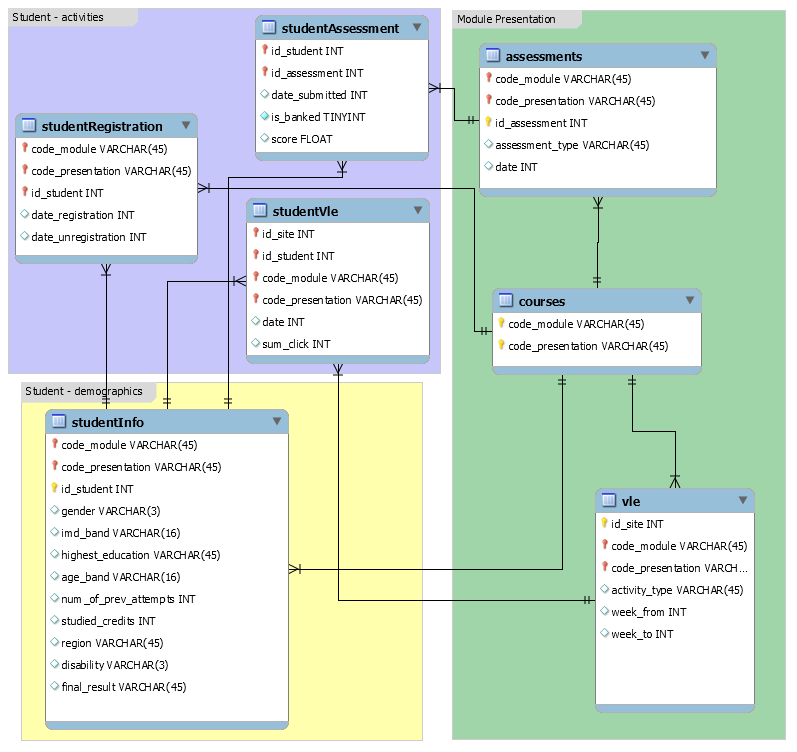
\includegraphics[scale=0.5]{db_model.png}
 \caption{OU learning analytics dataset relations}
 \label{fig:db_model}
 \end{figure}
 
\begin{figure}[h]
 \centering
 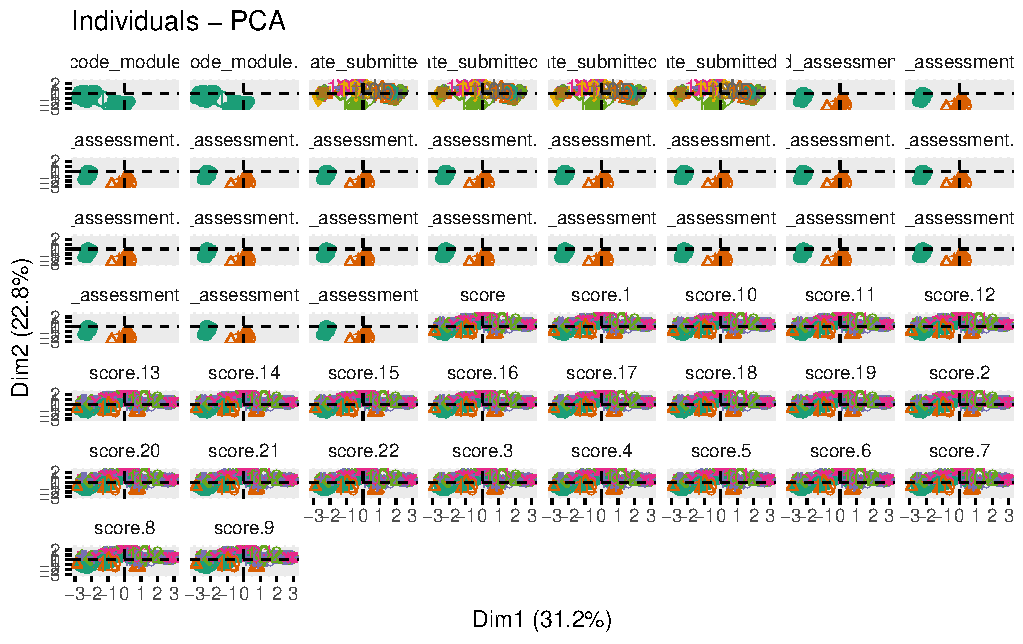
\includegraphics[scale=0.8]{PCA_Assessments_first50.pdf}
 \caption{PCA of student assessment attributes}
 \label{fig:pca}
 \end{figure}

\section{Results}

\section{Conclusions}


\hspace{1 cm}--- End

\newpage
\bibliographystyle{plain}
\bibliography{biblist}

\end{document}